\documentclass[12pt]{llncs}
\usepackage{tikz}
\usepackage{float}
\usepackage{amsmath}
\usepackage{graphicx}
\usepackage{subcaption}
\usepackage{multirow}
\usepackage{pgfplots}
\usepackage{pgfplotstable}
\usepackage{verbatim}
\usepackage[english]{babel}

\usetikzlibrary{calc}
\usepackage[
	backend=bibtex,
	style=numeric,
	sorting=none]{biblatex}
\addbibresource{references.bib}

\title{Mushroom classification with MobileNetV2 and Xception}
\author{Lorenzo Vainigli \\
lorenzo.vainigli@studio.unibo.it \\
matr. 0000842756}
\institute{Course of Machine Learning \\
Laurea Magistrale in Informatica \\
University of Bologna \\
A.Y. 2020-2021}
\date{\today}

\pagestyle{plain}

\begin{document}
{\def\addcontentsline#1#2#3{}\maketitle}

\begin{abstract}
The task of classifing mushrooms is difficult beacuse there are a lot of species to know and one might differ from another for very small details. This fact make it sometimes difficult for a human to recognize a species while looking at a photo of a mushroom. In this paper is presented a method to use two convolutional neural networks, MobileNetV2 and Xception, to try to solve this classification problem. Results we got shows that with machine learning we can handle this task but it requires a lot of work.
\end{abstract}

\begingroup
\let\clearpage\relax
\renewcommand{\contentsname}{}
\setcounter{tocdepth}{2} 
\tableofcontents
\endgroup

\section{Introduction}
The purpose of this project is to study and build a classifier that is able to recognize images of mushorooms and categorieze them. To do this we used two pre-trained convolutional neural networks that represent the state of the art: MobileNetV2 \cite{mobilenetv2} and Xception \cite{xception}. Both models were trained on ImageNet database \cite{imagenet}: MobileNetV2 achieved 71\% in top-1 accuracy and Xception achieved 79\% in the same metric. As regarding top-5 accuracy, Xception performs better with a score of 95\%, while MobileNet has a score of 90\%. The trade-off is that MobileNetV2 is six times smaller than Xception in memory storage.\\
The dataset was retrieved from \cite{fgvc}.

\section{Methods}
In this section we describe the process of use these models in our experiment. We begin with an analysis of the dataset to take a look at the data that we used for train, validation and test. Then we describe the steps followed to obtain the model for our purpose. \\
Briefly, we used the pre-trained convolutional layers of the two models to make a first training and test phase, we analized results and then we did another training and test phase, this time enabling the training of some convolutional layers. Details are explained in the next sections. We have done it both for ImageNetV2 and for Xception with 3, 10 and 20 classes of mushrooms from the dataset.

\subsection{Software}
This experiment was done using Python on the Google Colab platform \cite{colab} and Google GPUs. Tensorflow \cite{tensorflow} is the core tool used and the neural networks models are loaded from the Keras library.

\subsection{Dataset}
The image dataset is composed by an hierarchical structure of folders named with the category name of the images that they contains. Precisely each folder name has the format \texttt{ID\_super-category\_category}, so we use this information to associate these two properties (\textit{super-category} and \textit{category}) to the images, so each image has the label \texttt{super-category\_category}. This dataset is very large: it contains about 90,000 high resolution images belonging to about 1,500 classes. For our work we used 6,739 images belonging to 20 classes. Unfortunately, as shown in fig. \ref{fig:classes}, the dataset is very unbalanced; to create balanced sets without using class weights, we used the following amount of images depending on the number of classes: 414 if we use the first 3 classes, 340 if we use the first 10 classes and 255 if we use all the 20 classes.\\
There are also some annotation files in the dataset archive but we ignored it, since our purpose is to associate each image of mushroom to its category and no more.

\begin{figure}[h]
	\centering
	\includegraphics[width=\textwidth]{classes.png}
	\caption{Number of samples for each class sorted in descending order. The 20\textsuperscript{th} class has 38\% less images than the first class.}
	\label{fig:classes}
\end{figure}

\subsection{Image processing}
In this project we followed the official TensorFlow tutorial for transfer learning \cite{tf-transfer}. These guidelines suggests to add at the beginning of the model a \textit{random flip layer} and a \textit{random rotation layer} to perform augumentation on input images. In addition, an auxiliary input preprocessing layer was added because each Keras model expects a specific kind of input preprocessing. In our case these functions are:
\begin{itemize}
\item \texttt{tf.keras.applications.mobilenet\_v2.preprocess\_input} for MobileNetV2;
\item \texttt{tf.keras.applications.xception.preprocess\_input} for Xception.
\end{itemize}
As regarding image size, despite the models accept custom image sizes, we leave it as default: 224x224 for MobileNetV2 and 299x299 for Xception.

\subsection{Transfer learning}
We took advantage from the possibility to access the pre-trained models in a very simple way with Keras. Once we loaded one of the two models, we added a \textit{dense layer} to adapt it to our number of classes preceded by a \textit{pooling layer} and a \textit{dropout layer}. The complete architecture of the model is shown in fig. \ref{fig:model}.

\begin{figure}[h]
	\centering
    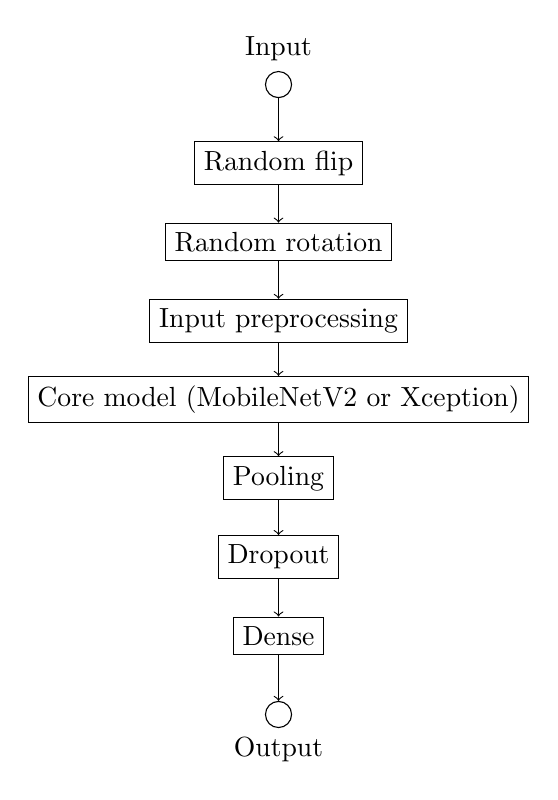
\begin{tikzpicture}
    \node[draw,circle,minimum size=3pt,label=above:Input] at (0,1) (in) {};
    \node[draw] at (0,0) (rf) {Random flip};
    \node[draw] at (0,-1) (rr) {Random rotation};
    \node[draw] at (0,-2) (pp) {Input preprocessing};
    \node[draw] at (0,-3) (m) {Core model (MobileNetV2 or Xception)};
    \node[draw] at (0,-4) (po) {Pooling};
    \node[draw] at (0,-5) (dr) {Dropout};
    \node[draw] at (0,-6) (de) {Dense};
    \node[draw,circle,minimum size=3pt,label=below:Output] at (0,-7) (out) {};
    \draw[->] (in.south) -- (rf.north) node {};
    \draw[->] (rf.south) -- (rr.north) node {};
    \draw[->] (rr.south) -- (pp.north) node {};
    \draw[->] (pp.south) -- (m.north) node {};
    \draw[->] (m.south) -- (po.north) node {};
    \draw[->] (po.south) -- (dr.north) node {};
    \draw[->] (dr.south) -- (de.north) node {};
    \draw[->] (de.south) -- (out.north) node {};
    \end{tikzpicture}
    \caption{Architecture of the model.}
    \label{fig:model}
\end{figure}

\subsection{Fine tuning}
As suggested in \cite{tf-transfer}, after the first training and evaluation of the model in which the training of the core model was disabled, a second training phase (fine tuning) has been performed to get better results. In fine tuning, some convolutional layers of the core model were unlocked for training and learning rate was decreased.

\subsection{Hyperparameters}
The experiments made shared the same settings of hyperparameters: the split between training-validation set and test set was 80\%-20\% as the split between training set and validation set; batch size was, as default, fixed to 32; learning rate is $10^{-4}$ for base training and $10^{-5}$ for fine tuning. Epochs were set to 100 for base training and 20 for fine tuning, but an early stopping with patience 10 was used to prevent overfitting.

\section{Results}
Table \ref{tab:accuracy} show that MobileNet performs better than Xception if we train the model with 3 classes, but if we choose 10 or 20 classes (and this means that the complexity is greater) Xception achieves better results. In figure \ref{fig:hist} we can clearly notice that the fine tuning helps a lot in the improvement of the model, especially if we have a high number of classes.\\
Considering the top-5 accuracy, instead, we can conclude that both models perform pretty well and that they achieve the same results.

\begin{table}[h]
\centering
\setlength{\tabcolsep}{5pt}
\def\arraystretch{1.2}
\begin{tabular}{ |c|c|c|c|c|c| } 
 \hline
 \multirow{2}{4em}{\textbf{Classes}} & \multirow{2}{6em}{\textbf{Samples per class}} & \multicolumn{2}{|c|}{\textbf{MobileNetV2}} & \multicolumn{2}{|c|}{\textbf{Xception}} \\ 
 \cline{3-6}
 & & \textbf{Top-1} & \textbf{Top-5} & \textbf{Top-1} & \textbf{Top-5} \\
 \hline 
 3 & 414 & 92\% & - & 90\% & - \\ 
 \hline 
 10 & 340 & 77\% & 98\% & 81\% & 98\% \\
 \hline 
 20 & 255 & 65\% & 95\% & 70\% & 95\% \\
 \hline
\end{tabular}
\caption{Result values for top-1 accuracy and top-5 accuracy.}
\label{tab:accuracy}
\end{table}

\begin{comment}
\begin{table}
\centering
\setlength{\tabcolsep}{5pt}
\def\arraystretch{1.2}
\begin{tabular}{ |c|c|c|c|c|c|c|c| } 
 \hline
 \multicolumn{3}{|c|}{\textbf{MobileNetV2}} & \multicolumn{3}{|c|}{\textbf{Xception}} \\ 
 \hline
 \textbf{Precision} & \textbf{Recall} & \textbf{F1 score} & \textbf{Precision} & \textbf{Recall} & \textbf{F1 score} \\
 \hline 
 92\% & 92\% & 92\% & 91\% & 90\% & 90\% \\ 
 \hline 
 78\% & 77\% & 77\% & 82\% & 81\% & 82\% \\
 \hline 
 66\% & 65\% & 65\% & 71\% & 70\% & 70\% \\
 \hline
\end{tabular}
\caption{Result values for precision, recall and F1 score.}
\label{tab:metrics}
\end{table}
\end{comment}

\begin{figure}[h]
\centering
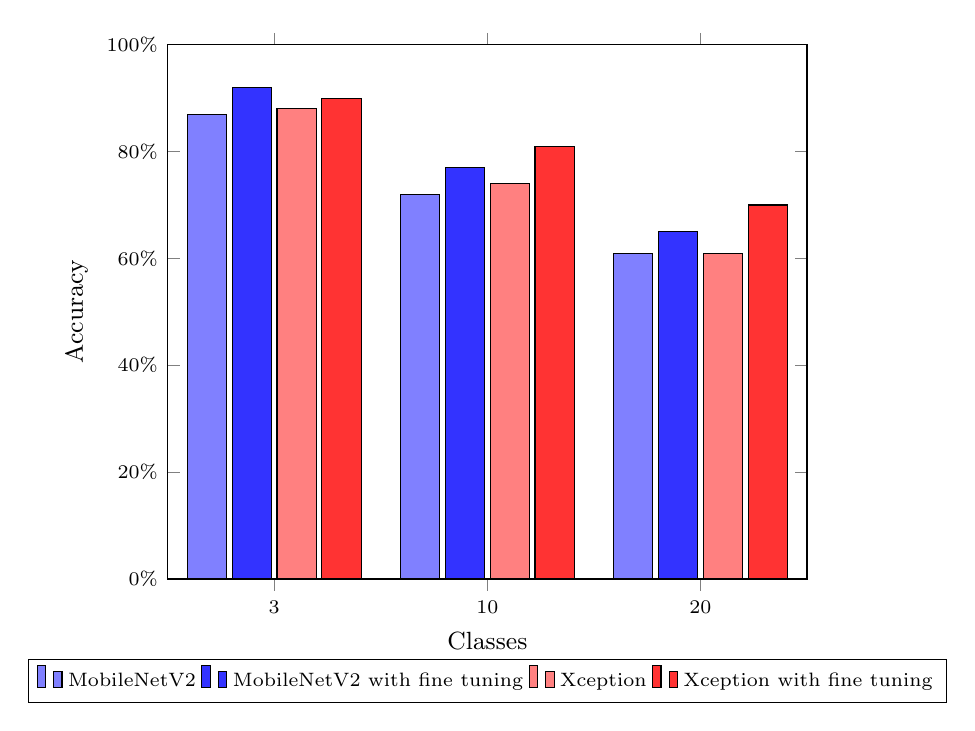
\begin{tikzpicture}
\begin{axis}[
	bar width=25,enlarge x limits=0.25,
	x tick label style={
        /pgf/number format/1000 sep=},
    ylabel={\small{Accuracy}},
    xlabel={\small{Classes}},
    yticklabel={\pgfmathparse{\tick}\pgfmathprintnumber{\pgfmathresult}\%},
    ymin=0,ymax=100,
    width = 0.8*\textwidth,
    legend style={
    	font=\scriptsize,
        at={(0.5,-0.15)},anchor=north
    },
    legend columns=-1,
    symbolic x coords={3,10,20},
    xtick=data,
    tick label style={font=\scriptsize},
    ybar,
    bar width = .5cm
]
\addplot [fill=blue!50] coordinates {(3,87)(10,72)(20,61)};
\addplot [fill=blue!80] coordinates {(3,92)(10,77)(20,65)};
\addplot [fill=red!50] coordinates {(3,88)(10,74)(20,61)};
\addplot [fill=red!80] coordinates {(3,90)(10,81)(20,70)};
\legend{MobileNetV2,MobileNetV2 with fine tuning,Xception,Xception with fine tuning}
\end{axis}
\end{tikzpicture}
\caption{Comparison of performances between MobileNetV2 and Xception.}
\label{fig:hist}
\end{figure}

\section{Discussion}
This work is only a basic application of two neural networks in image classification tasks and considering results achieved by these models with the 1,000 classes of ImageNet, the results on this dataset were not so good. We notice that with increasing the number of classes, the accuracy tends to decrease and 20 classes are a very few number. The dataset is not optimal and we can say that if we have a larger amount for each class, as the ImageNet dataset, results will be better.\\
Nevertheless, the dataset used is very interesting beacuse sometimes it will be very difficult for a human to recognize the species of a mushroom among all those that exist. Here the challenge is not to improve the models (even if there is room for improvement, it's more or less proven that they are good), but to improve the dataset with more samples.

\subsection*{Further directions}
The results shown were obtained training the two models with 3, 10 and 20 classes, but hyperparameters were fixed. It might be interesting to try different setting of hyperparameters to see how results change. Watching the learning curves of the training phase, we noticed that the limit of epochs can increased to obtain better accuracy.

\section{Conclusions}
In this paper was presented a method to use pre-trained neural networks to classify mushrooms. The work begun with an analysis of the dataset and then the model was implemented following the official guidelines. In addition to the classical training phase, a fine tuning phase was performed to achieve better performances. Results shows that models can correctly predict the true mushroom species for a given image with noticeable accuracy.

\printbibliography[title={References}]

\end{document}